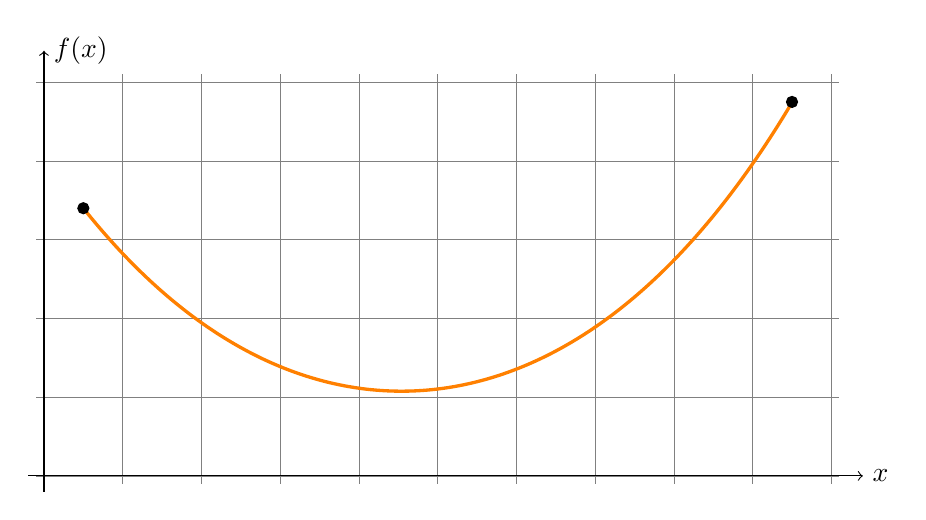
\begin{tikzpicture}[domain=-5:10]
    \draw[very thin,color=gray] (-0.1,-0.1) grid (10.1,5.1);
  
    \draw[->] (-0.2,0) -- (10.4,0) node[right] {$x$};
    \draw[->] (0,-0.2) -- (0,5.4) node[above, anchor=west] {$f(x)$};%~~~~~~~~~~\textcolor{orange}{--- Catenary curve}~~~~~~~~~~\textcolor{blue}{--- Parabolic curve}};


    \def\offsetx{-4}
    \def\ldomain{9}

    % Parabolic curve
    \def\aparab{0.15}
    \def\bparab{0}
    \def\cparab{1}
    % \draw[smooth, domain=0:\ldomain, samples=100, very thick, blue] plot ({\x+0.5}, {\aparab*(\x + \offsetx)*(\x + \offsetx) + \bparab*(\x + \offsetx) + \cparab});

    % End points
    \def\xaone{0.5}
    \pgfmathsetmacro\yaone{\aparab*(\offsetx)*(\offsetx) + \bparab*(\offsetx) + \cparab}
    \coordinate (Pa1) at (\xaone,\yaone);
    \pgfmathsetmacro\xatwo{\ldomain + 0.5}
    \pgfmathsetmacro\yatwo{\aparab*(\ldomain + \offsetx)*(\ldomain + \offsetx) + \bparab*(\ldomain + \offsetx) + \cparab}
    \coordinate (Pa2) at (\xatwo,\yatwo);

    % Catenary curve
    \def\C{0.26}
    \def\offsetx{-4.04}
    \pgfmathsetmacro\offsety{cosh((\offsetx)*\C)/\C - \yaone}
    \draw[smooth, domain=0:\ldomain, samples=100, very thick, orange] plot ({\x+0.5}, {cosh((\x + \offsetx)*\C)/\C - \offsety});

    \filldraw (Pa1) circle (2pt);
    \filldraw (Pa2) circle (2pt);

  \end{tikzpicture}